\section{Durchführung}
\label{sec:Durchführung}

\subsection{Überprüfung der Bragg-Bedingung}
Der Versuchsaufbau aus \ref{fig:Aufbau} wird verwendet.
Mit diesem und dem Messprogramm wurde ein fester Kristallwinkel von $\theta = \qty{14}{\degree}$ eingestellt.
Das Geiger-Müller Zählrohr soll dann in einem Winkelbereich von $\alpha_{GM}=\qty{26}{\degree}$ bis $\alpha_{GM}=\qty{30}{\degree}$ Messungen durchführen.
Dabei beträgt der Unterschied zwischen den einzelnen gemessenen Winkeln $\increment \alpha = \qty{0.2}{\degree}$.
Dies wird für alle weiteren Messungen so beibehalten.
Die Integrationszeit ist $\increment t=\qty{5}{\second}$.

\begin{figure}[H]
    \centering
    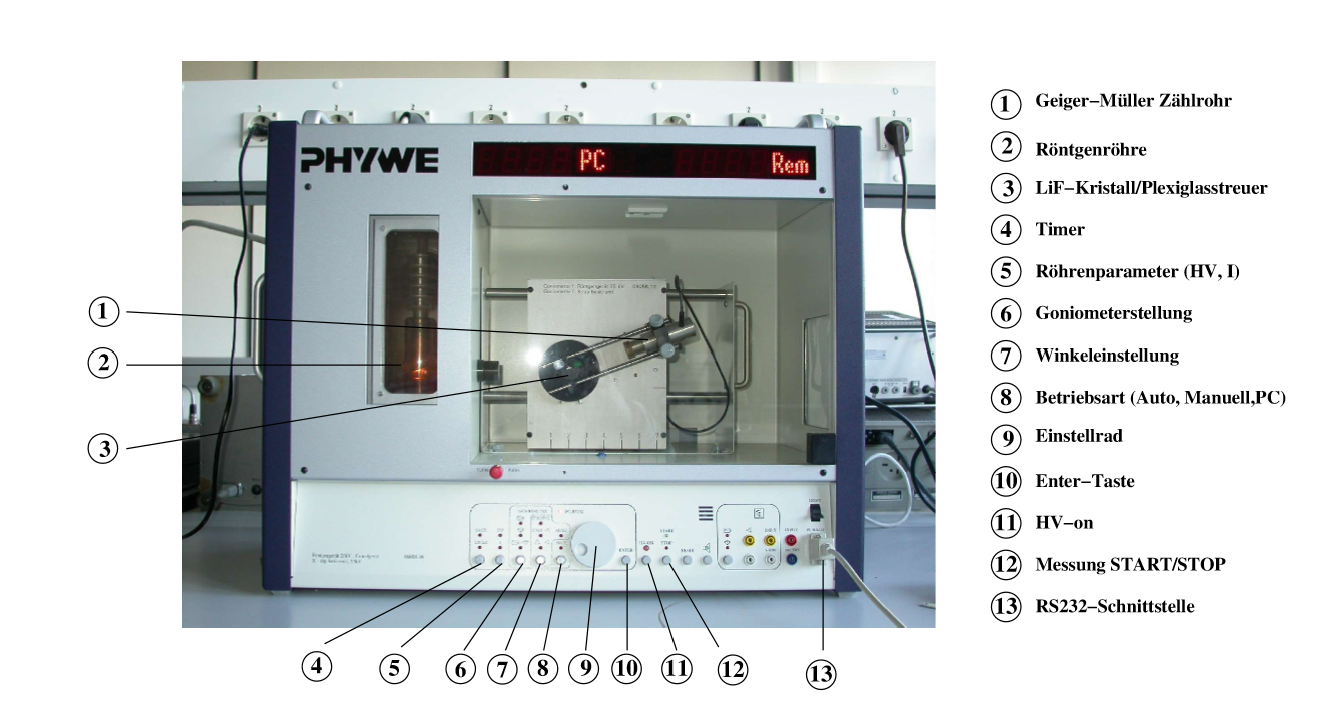
\includegraphics[width=\textwidth]{Bilder/Aufbau.png}
    \caption{Abgebildet ist ein Foto des Aufbaus des Versuches.}
    \label{fig:Aufbau}
\end{figure}

\subsection{Bestimmung des Emissionsspektrums einer CU-Röntgenröhre}
Für das Emissionsspektrum wird ein Winkelbereich von $\alpha_{GM}=\qty{4}{\degree}$ bis $\alpha_{GM}=\qty{26}{\degree}$ vermessen mit $\increment t=\qty{5}{\second}$.
Dabei wird der 2:1 Koppelmodus statt dem festen Kristallwinkel verwendet.

\subsection{Bestimmung der Absorbtionsspektren verschiedener Materialien}
Um die Absorbtionsspektren zu bestimmen, werden die Winkel für das jeweilige Material, die aus der Bragg-Bedingung folgen, genommen und in einem Winkelbereich von 
$\qty{-1}{\degree}$ bis $+ \qty{1}{\degree}$ um den Bragg Winkel gemessen.
Hier ist $\increment t=\qty{20}{\second}$.
Die Messung wird für die Materialen Zink, Gallium, Brom, Strontium und Zirkonium.
Dabei sind die Bragg-Winkel und die Orndungszahlen in \ref{tab:tabelle} angegeben.

\begin{table}
    \centering
    \caption{Augelistet sind die Elemente, für die die Emissionsspektren bestimmt werden und deren Orndungszahl ung Bragg-Winkel.}
    \label{tab:tabelle}
    \sisetup{table-format=1.1, per-mode=reciprocal}
    \begin{tblr}{
        colspec = {S[table-format=2.0] S[table-format=2.0] S[table-format=2.1]},
        row{1} = {guard, mode=math},
      }
      \toprule
      Element & Z &\alpha \mathbin{/} \unit{\degree} \\
      \midrule
        Zn & 30& 18.7\\
        Ga & 31& 17.3\\
        Br & 35& 13.2\\
        Sr & 38& 11.1\\
        Zr & 40& 9.9 \\
      \bottomrule
    \end{tblr}
  \end{table}